\begin{figure}[t]
\centering
    \centering
    \begin{minipage}{0.63\textwidth}
        \centering
        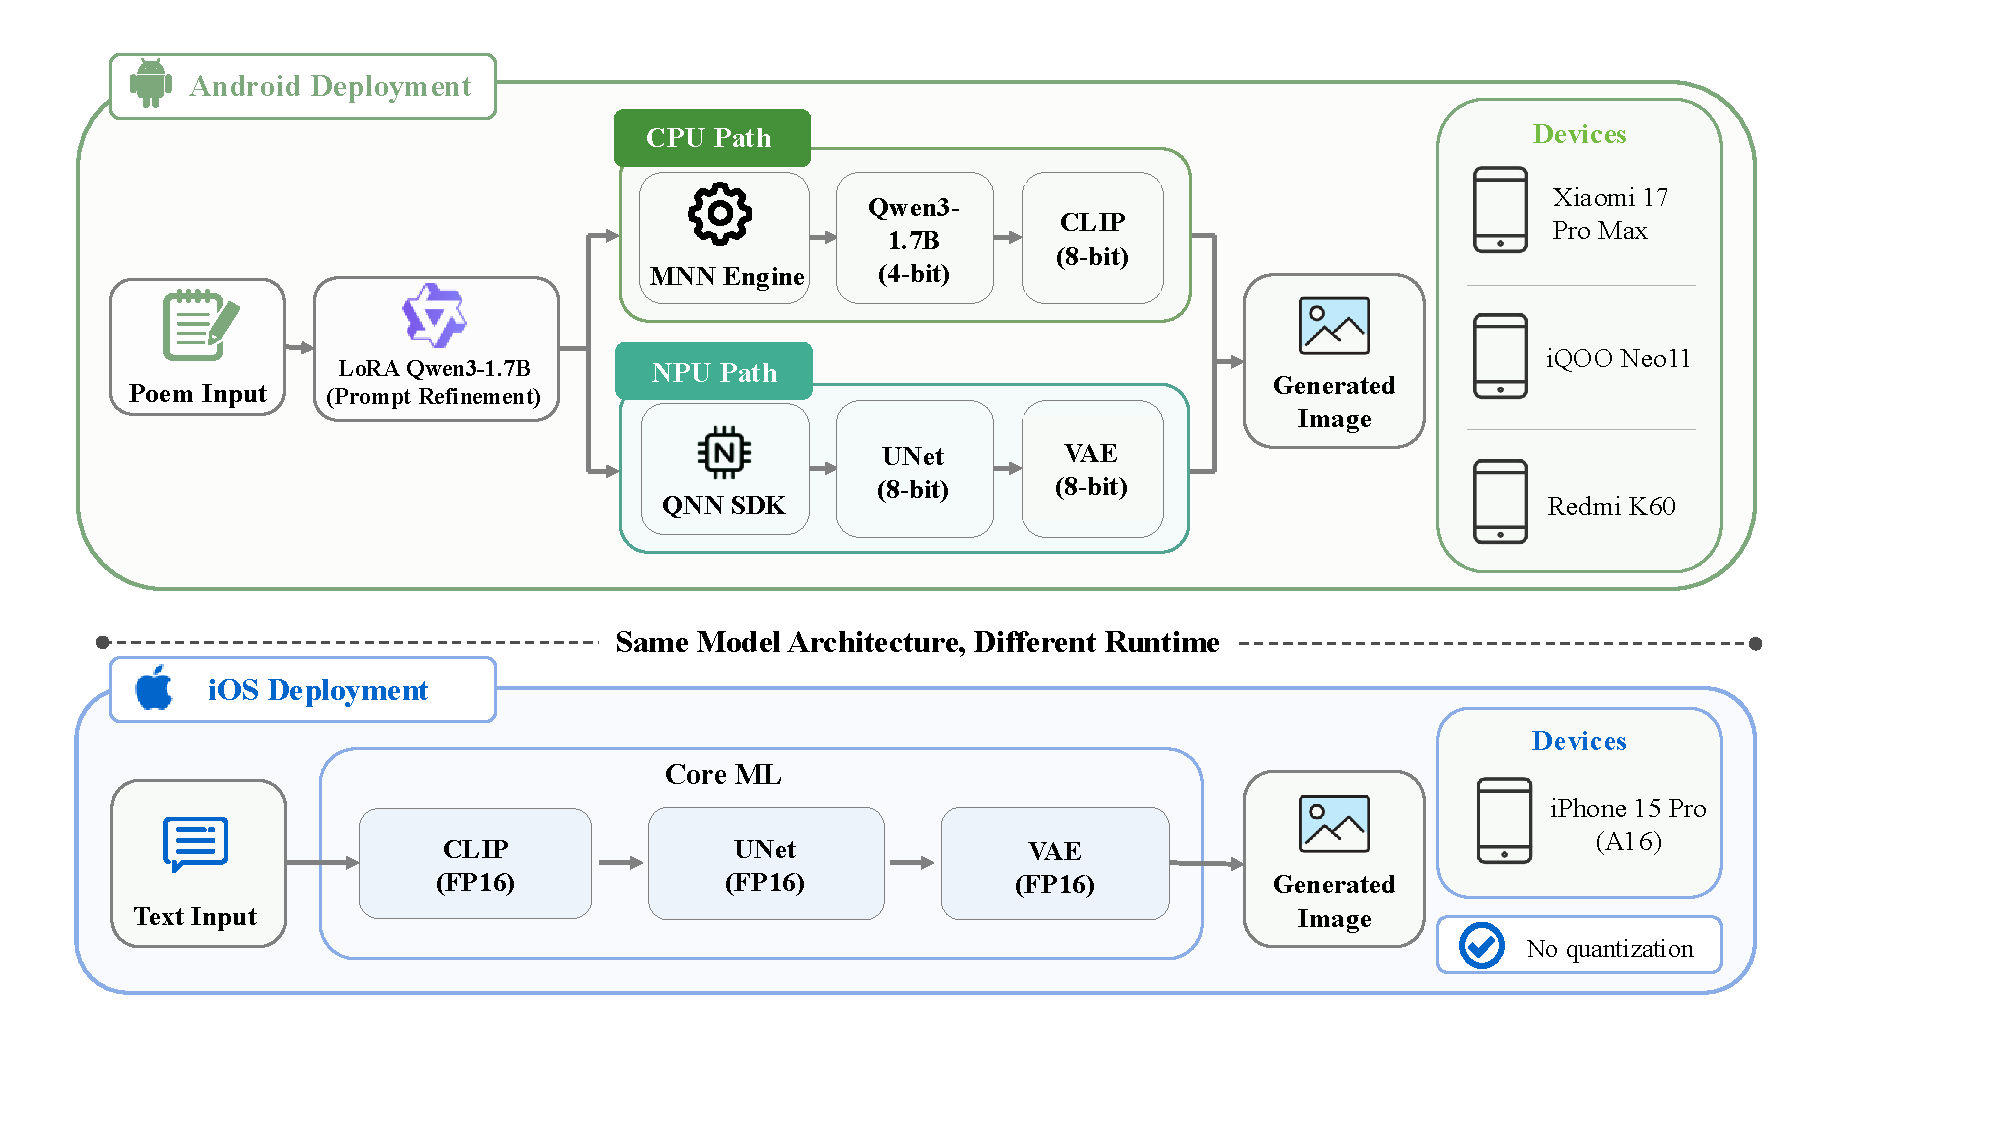
\includegraphics[width=\textwidth]{figures/figures/fig08.pdf}
        \caption{\textbf{Heterogeneous deployment architecture across Android and iOS platforms.} On Android, the pipeline is partitioned between CPU (MNN engine for language model and text encoding) and NPU (QNN for U-Net and VAE decoding). On iOS, all diffusion modules run on Core ML in FP16 precision without additional quantization.}
        \label{fig:deployment_architecture}
    \end{minipage}
    \hfill  % 在两个子图间插入弹性空白，实现分离
    \begin{minipage}{0.33\textwidth}
        \centering
        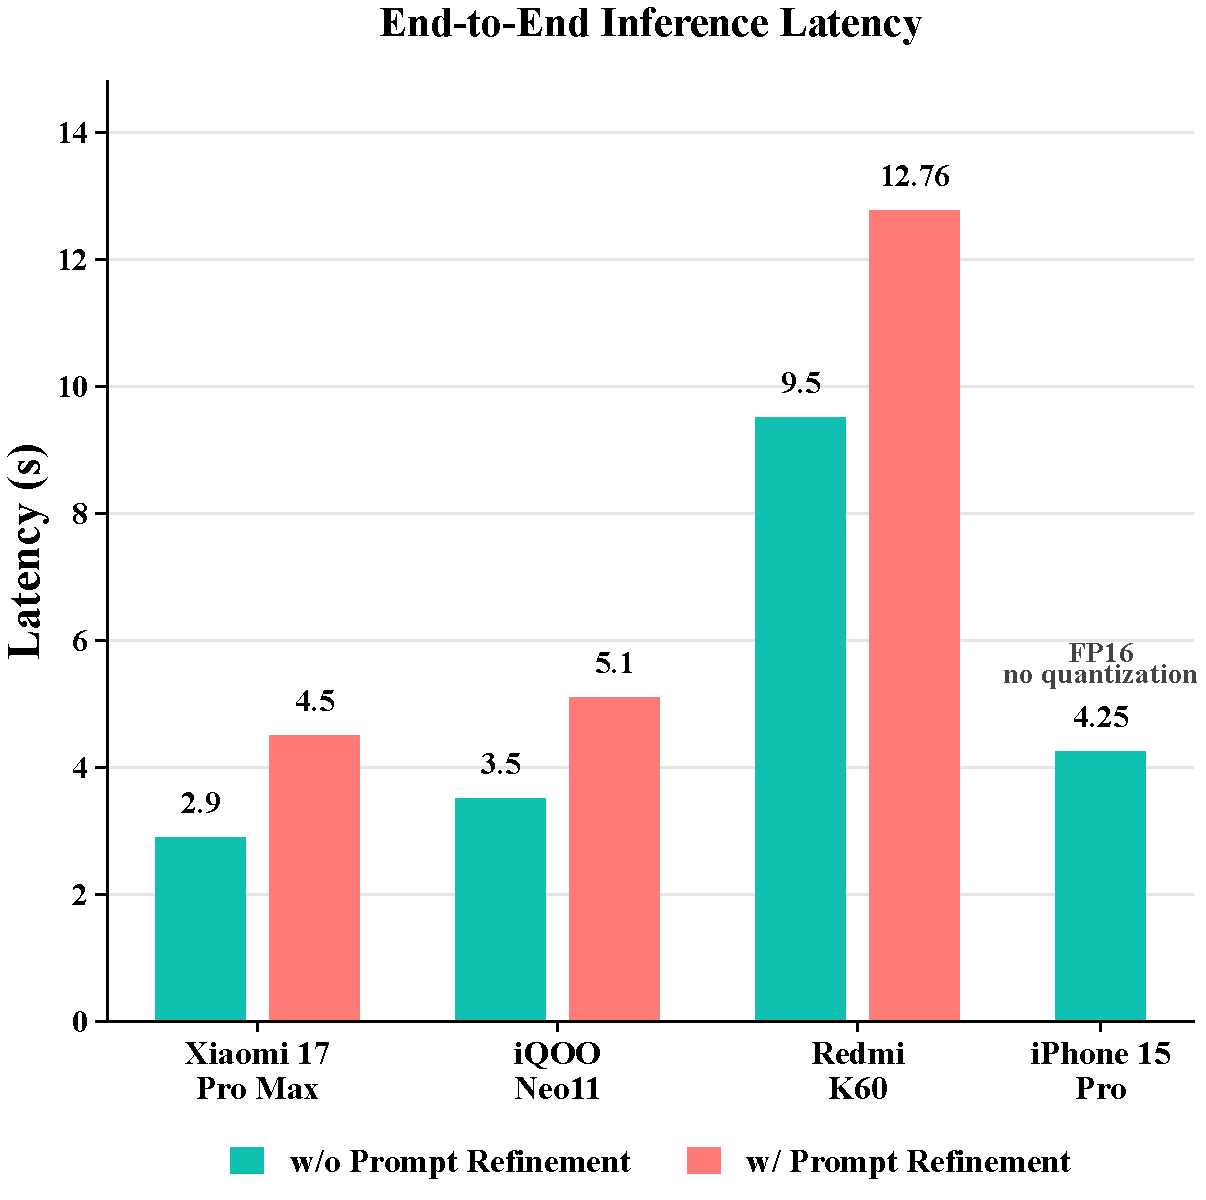
\includegraphics[width=\textwidth]{figures/figures/fig09.pdf}
        \caption{\textbf{Mobile inference latency.} Xiaomi 17 Pro Max completes the full pipeline in 4.5\,s; iPhone 15 Pro runs the CLIP--U-Net--VAE branch in 4.25\,s (FP16).}
        \label{fig:latency_comparison}
    \end{minipage}
\end{figure}

\section{Edge Device Deployment}

To enable fully on-device T2I generation, we adopt a heterogeneous execution pipeline shown in Fig.~\ref{fig:deployment_architecture} that separates text processing from image synthesis. In the poetry application, a LoRA-tuned Qwen3-1.7B language model~\cite{qwen3technicalreport} first rewrites the input poem into a clearer, generation-oriented description. The refined prompt then feeds into the core diffusion pipeline, which comprises three modules: a Chinese CLIP text encoder~\cite{chinese-clip}, a denoising network, and a VAE decoder.

These components exhibit substantially different computational characteristics and are therefore not mapped to a single runtime backend. Instead, control-dominant and text-heavy modules execute on the CPU via lightweight inference engines, while the computationally intensive denoising and decoding stages are offloaded to dedicated neural accelerators whenever available. This design minimizes cloud dependence, preserves data locality, and enables responsive interactive generation on mobile devices. Recent advances in low-bit quantization for both diffusion~\cite{li2023qdiffusion} and transformer~\cite{wu2023int4,liu2025quantization_survey} models informed our deployment strategy.

\subsection{Adaptation Solutions for Snapdragon-based Android devices}

% The Android deployment adopts a heterogeneous runtime strategy that partitions the generation pipeline across CPU and NPU backends according to the computational characteristics of each module. Language-model-based prompt refinement and text encoding run on the CPU via the MNN engine, while arithmetic-intensive U-Net denoising and VAE decoding are offloaded to the Qualcomm NPU through the QNN SDK. We validate this partitioning across three Snapdragon-based devices spanning multiple hardware generations.
% For Android deployment, we adopt a heterogeneous CPU--NPU runtime strategy. Prompt refinement and text encoding run on the CPU with MNN, while the computation-intensive U-Net denoising and VAE decoding are offloaded to the Qualcomm NPU via QNN SDK. This strategy is validated on three Snapdragon-based devices across different hardware generations.
The Android deployment adopts a heterogeneous runtime strategy that partitions the generation pipeline across CPU and NPU backends according to the characteristics of each module. Prompt refinement and text encoding run on the CPU via the MNN engine, while arithmetic-intensive U-Net denoising and VAE decoding are offloaded to the Qualcomm NPU through the QNN SDK. We validate this partitioning across three Snapdragon-based devices spanning multiple hardware generations.

We use the Snapdragon\textsuperscript{\textregistered} 8 Elite Gen 5
Mobile Platform (SM8850) as the primary Android acceleration target and
treat the other Snapdragon devices as cross-generation validation platforms.
In this setup, model execution is not merely a direct port of the desktop
diffusion pipeline. Instead, the diffusion branch is compiled into
QNN-compatible artifacts and executed through the HTP backend, whereas
the text branch remains on the CPU-side MNN runtime. The Android application
identifies the target SoC at runtime and loads the corresponding U-Net and
VAE binaries, allowing the same high-level model architecture to be preserved
while the low-level execution path is specialized for each Snapdragon platform.

\subsubsection{Device platforms and runtime partitioning}
% The Android implementation is validated on three Snapdragon-based smartphones spanning three hardware generations: Xiaomi 17 Pro Max (SM8850, Android 16), iQOO Neo11 (SM8750, Android 16), and Redmi K60 (SM8475, Android 15). The prompt-refinement model, namely the LoRA-tuned Qwen3-1.7B, executes on the CPU through the MNN~\cite{alibaba2020mnn} inference engine with 4-bit quantization. The CLIP text encoder also executes on the CPU through MNN with 8-bit quantization. By contrast, the two computationally dominant diffusion modules, U-Net and VAE, are deployed through the Qualcomm AI Engine Direct SDK~\cite{qnn} and executed on the NPU with 8-bit quantization.
We validate the Android implementation on three Snapdragon-based smartphones across different hardware generations: Xiaomi 17 Pro Max (SM8850, Android 16), iQOO Neo11 (SM8750, Android 16), and Redmi K60 (SM8475, Android 15). The LoRA-tuned Qwen3-1.7B prompt-refinement model and CLIP text encoder run on the CPU via MNN~\cite{alibaba2020mnn} with 4-bit and 8-bit quantization, respectively. In contrast, the computation-heavy U-Net and VAE are deployed on the NPU via Qualcomm AI Engine Direct SDK~\cite{qnn} with 8-bit quantization.

We select this runtime partitioning for two reasons. First, U-Net denoising and VAE decoding dominate arithmetic intensity and benefit most from hardware acceleration. Second, the language model and the text encoder benefit from the portability and lower integration overhead of a CPU-side runtime. In deployment, all model files are hosted remotely, downloaded into an application-specific directory, and subsequently loaded through native C++ interfaces for local inference. On flagship devices, the end-to-end application generates a high-quality image from a poem in approximately 5 seconds.

\subsubsection{Model conversion, packaging, and runtime orchestration}

% \begin{figure}[t]
%     \centering
%     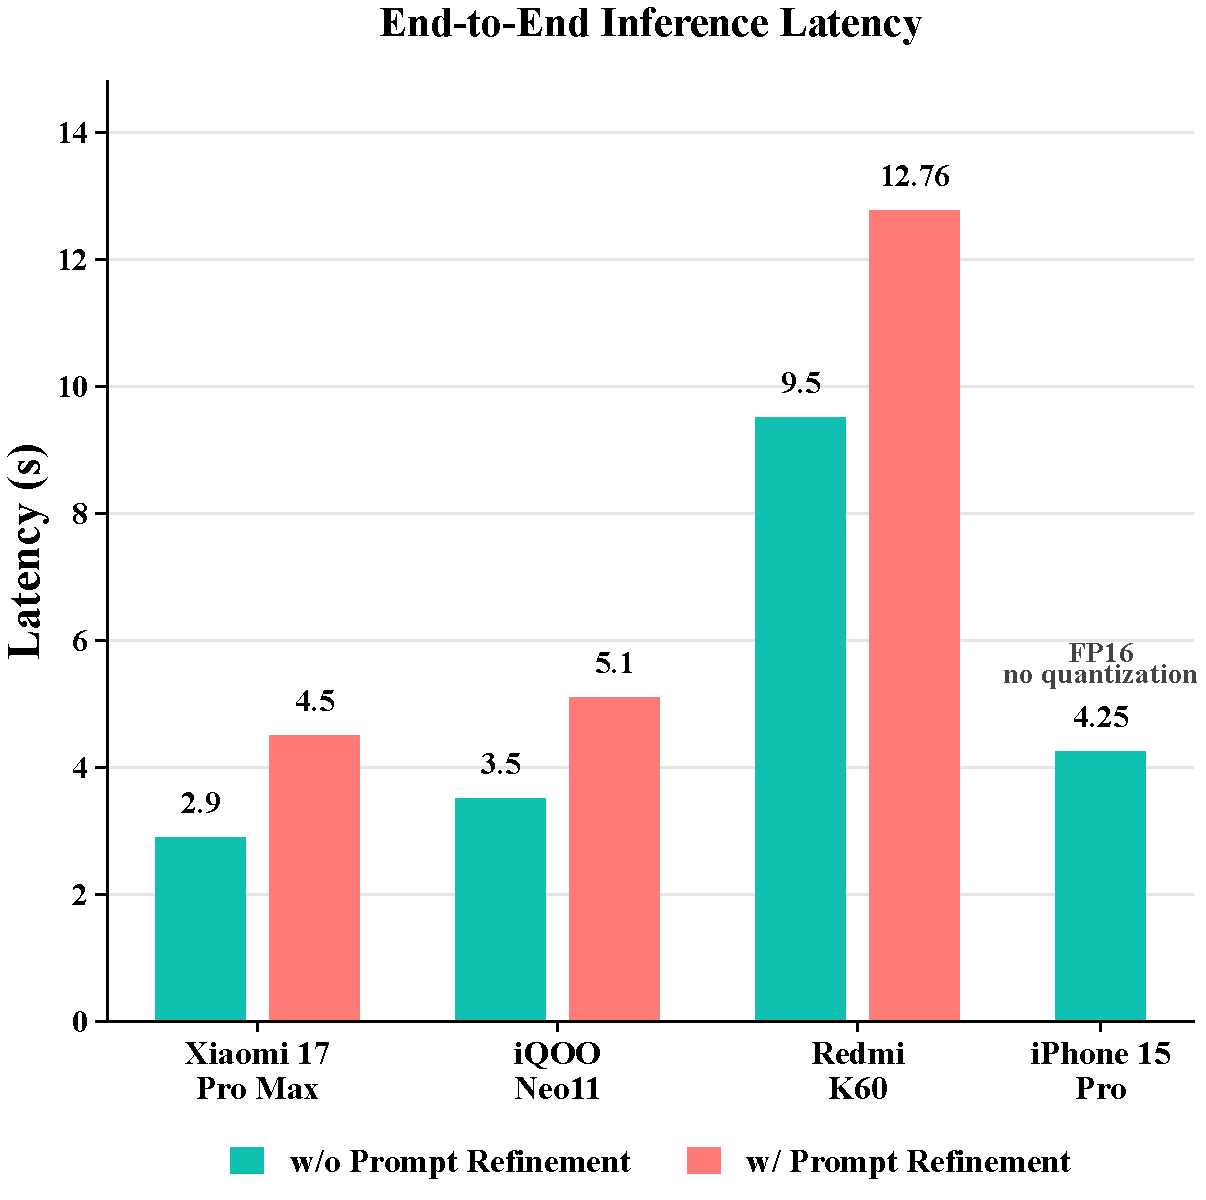
\includegraphics[width=0.25\textwidth]{figures/figures/fig09.pdf}
%     \caption{\textbf{Mobile inference latency.} Xiaomi 17 Pro Max completes the full pipeline in 4.5\,s; iPhone 15 Pro runs the CLIP--U-Net--VAE branch in 4.25\,s (FP16).}
%     \label{fig:latency_comparison}
%     \vspace{-6pt}
% \end{figure}

% For the diffusion branch, we export the PyTorch checkpoints of U-Net and VAE to ONNX and subsequently transform them into QNN-compatible artifacts. The conversion pipeline generates platform-specific intermediate files and runtime context binaries, thereby enabling NPU execution through the HTP backend. In practice, the Android application selects hardware-adapted U-Net and VAE binaries based on chip identification while preserving a unified application interface.
For the diffusion branch, U-Net and VAE checkpoints are exported from PyTorch to ONNX and converted into QNN-compatible artifacts for NPU execution via the HTP backend. The Android application selects chip-specific U-Net and VAE binaries according to device identification while maintaining a unified application interface.

For the prompt-refinement model and the CLIP text encoder, we adopt the MNN deployment path. We convert the CLIP encoder from ONNX to MNN with 8-bit quantization and export the LoRA-tuned Qwen3-1.7B model through the MNN language-model pipeline with 4-bit compression. At runtime, the application downloads the required model files from cloud object storage into the local app sandbox and initializes them through native C++ interfaces. The execution order remains fixed: poem input, prompt refinement, CLIP encoding, iterative U-Net denoising, VAE decoding, and final image output.

% \subsubsection{Stability, resource usage, and latency}

% We characterize system stability from three complementary perspectives: hardware adaptation stability, performance stability, and long-run resource stability. On the hardware side, we convert the NPU-side U-Net and VAE models separately for each Snapdragon platform, and the application dynamically loads the hardware-compatible binaries after identifying the target chip. On the CPU side, the same MNN models are reused across chips without cross-platform compatibility issues.

% We evaluate performance stability through repeated measurements of language-model first-token latency and throughput, CLIP text-encoding time, U-Net single-step denoising latency, and VAE image-decoding time. We examine resource stability during continuous operation, including 100 consecutive image-generation runs, by tracking CPU utilization and memory usage. Across all evaluated Android devices, the application remains operational without abnormal interruption, and the measured latency and memory footprint remain within a stable range.

% Tab.~\ref{tab:android_deployment_results} presents the Android deployment results across three Snapdragon-based mobile platforms, including latency and memory usage with and without prompt refinement.
\subsubsection{Stability, resource usage, and latency}

We evaluate Android deployment stability from three aspects: hardware adaptation, runtime performance, and long-run resource usage. For hardware adaptation, the NPU-side U-Net and VAE binaries are converted separately for each Snapdragon platform and dynamically loaded according to the detected chip, while the CPU-side MNN models are shared across devices.

% For runtime stability, we repeatedly measure language-model first-token latency and throughput, CLIP encoding time, U-Net single-step denoising latency, and VAE decoding time. We further conduct 100 consecutive image-generation runs to monitor CPU utilization and memory usage. Across all evaluated Android devices, the application remains operational without abnormal interruption, and both latency and memory footprint stay within a stable range. Tab.~\ref{tab:android_deployment_results} reports latency and memory usage with and without prompt refinement across the three Snapdragon-based platforms.
For runtime stability, we repeatedly measure language-model first-token latency and throughput, CLIP encoding time, U-Net single-step denoising latency, and VAE decoding time. We also conduct 100 consecutive image-generation runs to monitor CPU utilization and memory usage. Across all evaluated Android devices, the application remains operational without abnormal interruption, with latency and memory footprint staying within stable ranges. Tab.~\ref{tab:android_deployment_results} reports latency and memory usage with and without prompt refinement across the three Snapdragon-based platforms.

% \begin{table}[t]
% \centering
% \caption{Android deployment performance on Snapdragon-based mobile platforms.}
% \label{tab:android_deployment_results}
% \small
% \setlength{\tabcolsep}{4pt}
% \renewcommand{\arraystretch}{1.18}
% \begin{tabularx}{\linewidth}{
% @{}
% >{\raggedright\arraybackslash}p{2.75cm}
% >{\raggedright\arraybackslash}X
% >{\centering\arraybackslash}p{1.75cm}
% >{\centering\arraybackslash}p{1.05cm}
% >{\centering\arraybackslash}p{1.05cm}
% >{\centering\arraybackslash}p{1.15cm}
% >{\centering\arraybackslash}p{1.15cm}
% @{}
% }
% \toprule
% \multirow{2}{*}{Device} &
% \multirow{2}{*}{Mobile Platform} &
% \multirow{2}{*}{OS} &
% \multicolumn{2}{c}{Latency} &
% \multicolumn{2}{c}{Memory} \\
% \cmidrule(lr){4-5}
% \cmidrule(l){6-7}
% & & &
% w/o Ref. &
% w/ Ref. &
% w/o Ref. &
% w/ Ref. \\
% \midrule

% Xiaomi17 Pro Max &
% Snapdragon\textsuperscript{\textregistered} 8 Elite Gen 5 (SM8850) &
% Android 16 &
% 2.9~s &
% 4.5~s &
% 200~MB &
% 1.3~GB \\

% iQOO Neo11 &
% Snapdragon\textsuperscript{\textregistered} 8 Elite (SM8750) &
% Android 16 &
% 3.5~s &
% 5.1~s &
% 200~MB &
% 1.3~GB \\

% Redmi K60 &
% Snapdragon\textsuperscript{\textregistered} 8+ Gen 1 (SM8475) &
% Android 15 &
% 9.5~s &
% 12.7~s &
% 180~MB &
% 1.3~GB \\

% \bottomrule
% \end{tabularx}
% \end{table}

% \begin{table}[t]
% \centering
% \caption{Android deployment performance on Snapdragon-based mobile platforms.}
% \label{tab:android_deployment_results}
% \footnotesize
% \setlength{\tabcolsep}{4pt}
% \renewcommand{\arraystretch}{1.12}

% \begin{tabular*}{0.96\linewidth}{@{\extracolsep{\fill}}lllcccc@{}}
% \toprule
% \textbf{Device} &
% \textbf{Mobile Platform} &
% \textbf{OS} &
% \multicolumn{2}{c}{\textbf{Latency}} &
% \multicolumn{2}{c}{\textbf{Memory}} \\
% \cmidrule(lr){4-5}
% \cmidrule(lr){6-7}
% & & &
% \textbf{w/o Ref.} &
% \textbf{w/ Ref.} &
% \textbf{w/o Ref.} &
% \textbf{w/ Ref.} \\
% \midrule

% Xiaomi 17 Pro Max &
% Snap. 8 Elite Gen 5 &
% Android 16 &
% 2.9 s &
% 4.5 s &
% 200 MB &
% 1.3 GB \\

% iQOO Neo11 &
% Snap. 8 Elite &
% Android 16 &
% 3.5 s &
% 5.1 s &
% 200 MB &
% 1.3 GB \\

% Redmi K60 &
% Snap. 8+ Gen 1 &
% Android 15 &
% 9.5 s &
% 12.7 s &
% 180 MB &
% 1.3 GB \\

% \bottomrule
% \end{tabular*}

% \renewcommand{\arraystretch}{1.0}
% \end{table}
\begin{table}[t]
\centering
\caption{Android deployment performance on Snapdragon-based mobile platforms.}
\label{tab:android_deployment_results}
\footnotesize
\setlength{\tabcolsep}{4pt}
\renewcommand{\arraystretch}{1.10}

\hspace*{-0.020\linewidth}%
\begin{tabular*}{0.98\linewidth}{@{\extracolsep{\fill}}lllcccc@{}}
\toprule
\textbf{Device} &
\textbf{Mobile Platform} &
\textbf{OS} &
\textbf{Lat. w/o Ref.} &
\textbf{Lat. w/ Ref.} &
\textbf{Mem. w/o Ref.} &
\textbf{Mem. w/ Ref.} \\
\midrule

Xiaomi 17 Pro Max &
Snap. 8 Elite Gen 5 &
Android 16 &
2.9 s &
4.5 s &
200 MB &
1.3 GB \\

iQOO Neo11 &
Snap. 8 Elite &
Android 16 &
3.5 s &
5.1 s &
200 MB &
1.3 GB \\

Redmi K60 &
Snap. 8+ Gen 1 &
Android 15 &
9.5 s &
12.7 s &
180 MB &
1.3 GB \\

\bottomrule
\end{tabular*}

\renewcommand{\arraystretch}{1.0}
\end{table}

\subsection{Cross-Platform Deployment Mapping}

% A notable characteristic of this deployment is that the same high-level model decomposition can be preserved across mobile ecosystems even though the runtime stacks differ substantially. On Android, we obtain fine-grained control by assigning U-Net and VAE to QNN-based NPU execution and assigning the language model and CLIP encoder to MNN on the CPU. On iOS, the validated deployment currently focuses on the CLIP--U-Net--VAE generation branch, where all three models are converted into Core ML packages and invoked through a Swift application.
% This deployment preserves the same high-level model decomposition across mobile ecosystems despite different runtime stacks. On Android, U-Net and VAE run on the NPU via QNN, while the language model and CLIP encoder run on the CPU via MNN. On iOS, the validated deployment focuses on the CLIP--U-Net--VAE branch, with all three models converted to Core ML packages and invoked through a Swift application. Tab.~\ref{tab:correspondence_android_ios} summarizes the component-level correspondence between the Android and iOS deployment pipelines, highlighting how the same high-level model decomposition is mapped to different runtime stacks.
This deployment preserves the same high-level model decomposition across mobile ecosystems despite different runtime stacks. On Android, U-Net and VAE run on the NPU via QNN, while the language model and CLIP encoder run on the CPU via MNN. On iOS, the validated deployment focuses on the CLIP--U-Net--VAE branch, with all three models converted to Core ML packages and invoked through a Swift application. Tab.~\ref{tab:correspondence_android_ios} reports the component-level correspondence between the two deployment pipelines.

% \begin{table}[t]
%     \centering
%     \caption{Correspondence between Android and iOS deployment components.}
%     \label{tab:correspondence_android_ios}
%     \small
%     \setlength{\tabcolsep}{5pt}
%     \renewcommand{\arraystretch}{1.18}
%     \begin{tabularx}{\textwidth}{
%         >{\raggedright\arraybackslash}p{0.24\textwidth}
%         >{\raggedright\arraybackslash}X
%         >{\raggedright\arraybackslash}X
%     }
%         \toprule
%         \textbf{Pipeline component} & \textbf{Android implementation} & \textbf{iOS implementation} \\
%         \midrule
%         Prompt refinement% (Qwen3-1.7B) 
%         & MNN, CPU, 4-bit compressed model 
%         & Not included in the current validated iOS setup \\
%         CLIP text encoder 
%         & MNN, CPU, 8-bit quantization 
%         & Core ML, FP16 \\
%         U-Net denoiser 
%         & QNN, NPU, 8-bit quantization 
%         & Core ML, FP16 \\
%         VAE decoder 
%         & QNN, NPU, 8-bit quantization 
%         & Core ML, FP16 \\
%         Model delivery 
%         & Remote download into the app sandbox 
%         & Loaded by the Swift app through Core ML model packages \\
%         Orchestration layer 
%         & Native C++ Android application 
%         & Swift iOS application with Core ML inference \\
%         \bottomrule
%     \end{tabularx}
%     \renewcommand{\arraystretch}{1.0}
%     \setlength{\tabcolsep}{6pt}
% \end{table}
% \begin{table}[t]
%     \centering
%     \caption{Correspondence between Android and iOS deployment components.}
%     \label{tab:correspondence_android_ios}
%     \footnotesize
%     \setlength{\tabcolsep}{4pt}
%     \renewcommand{\arraystretch}{1.12}

%     \begin{tabular*}{0.96\linewidth}{@{\extracolsep{\fill}}lll@{}}
%         \toprule
%         \textbf{Component} & \textbf{Android} & \textbf{iOS} \\
%         \midrule
%         Prompt refinement & MNN CPU, 4-bit & Not used in validated setup \\
%         CLIP text encoder & MNN CPU, INT8 & Core ML, FP16 \\
%         U-Net denoiser & QNN NPU, INT8 & Core ML, FP16 \\
%         VAE decoder & QNN NPU, INT8 & Core ML, FP16 \\
%         Model delivery & Remote download to app sandbox & Core ML model packages \\
%         Orchestration layer & Native C++ Android app & Swift app with Core ML \\
%         \bottomrule
%     \end{tabular*}

%     \renewcommand{\arraystretch}{1.0}
%     \setlength{\tabcolsep}{6pt}
% \end{table}
\begin{table}[t]
    \centering
    \caption{Correspondence between Android and iOS deployment components.}
    \label{tab:correspondence_android_ios}
    \footnotesize
    \setlength{\tabcolsep}{4pt}
    \renewcommand{\arraystretch}{1.12}

    \begin{tabularx}{0.96\linewidth}{
        @{}
        >{\raggedright\arraybackslash}p{0.28\linewidth}
        >{\raggedright\arraybackslash}X
        >{\raggedright\arraybackslash}X
        @{}
    }
        \toprule
        \textbf{Component} & \textbf{Android} & \textbf{iOS} \\
        \midrule
        Prompt refinement & MNN CPU, 4-bit & Not used in validated setup \\
        CLIP text encoder & MNN CPU, INT8 & Core ML, FP16 \\
        U-Net denoiser & QNN NPU, INT8 & Core ML, FP16 \\
        VAE decoder & QNN NPU, INT8 & Core ML, FP16 \\
        Model delivery & Remote download to app sandbox & Core ML model packages \\
        Orchestration layer & Native C++ Android app & Swift app with Core ML \\
        \bottomrule
    \end{tabularx}

    \renewcommand{\arraystretch}{1.0}
    \setlength{\tabcolsep}{6pt}
\end{table}

\subsection{iOS Deployment Adaptation}

% On the iOS side, the deployment leverages Apple's Core ML framework as a unified runtime for the CLIP text encoder, U-Net denoiser, and VAE decoder. Unlike the Android implementation, which partitions execution across MNN and QNN, the iOS pipeline consolidates all three diffusion modules into a single inference stack via \texttt{coremltools}. The validated configuration operates in FP16 precision without additional quantization.
% On the iOS side, the deployment uses Apple's Core ML framework as a unified runtime for the CLIP text encoder, U-Net denoiser, and VAE decoder. Unlike the Android implementation, which partitions execution across MNN and QNN, the iOS pipeline consolidates all three diffusion modules into a single inference stack via \texttt{coremltools}. The validated configuration runs in FP16 precision without additional quantization.
On iOS, Apple's Core ML framework provides a unified runtime for the CLIP text encoder, U-Net denoiser, and VAE decoder. Unlike Android's MNN--QNN partitioned execution, the iOS pipeline consolidates all three diffusion modules into a single \texttt{coremltools}-based inference stack, running in FP16 precision without additional quantization.

\subsubsection{Model export and Core ML conversion}

In the validated iOS deployment, the iOS branch consists of three core image-generation modules: CLIP, U-Net, and VAE. We first export each module to ONNX, after which the ONNX graphs are converted into \texttt{.mlpackage} format using \texttt{coremltools}. This conversion path preserves the modular boundaries of the original diffusion system and aligns the deployment with Apple’s native model format.

At the current stage, the validated iOS implementation focuses on the CLIP--U-Net--VAE image-generation stack rather than the auxiliary Qwen3-1.7B prompt-refinement model used in the Android pipeline. We note this distinction explicitly because the reported iPhone measurements correspond to the deployed three-model image-generation branch. This branch represents the computationally dominant part of the system and therefore provides a meaningful validation of Apple-side edge deployment.

% \begin{table}[t]
%     \centering
%     % \caption{On-device hardware profiling of the denoising network at $1024\times1024$ resolution across flagship mobile platforms. Mainstream models (SD~1.5, SDv2.1) fail to execute on mobile devices due to excessive memory requirements or impractical latency.}
%     \caption{UNet-only on-device profiling at $1024\times1024$ resolution across flagship mobile platforms. The reported latency measures only the 4-step denoising branch of the distilled JuZhou 1.0 model. CLIP text encoding, VAE decoding, prompt refinement, and application-level orchestration are excluded. Mainstream baselines such as SD 1.5 and SDv2.1 fail to execute under the same mobile profiling setup because of excessive memory requirements or impractical latency.}
%     \label{tab:hardware_profiling}
%     \small
%     \setlength{\tabcolsep}{3pt}
%     \renewcommand{\arraystretch}{1.15}
%     \begin{tabular}{lcccccccc}
%         \toprule
%         \textbf{Model} 
%         & \textbf{\begin{tabular}[c]{@{}c@{}}Denoiser\\+ VAE Dec.\end{tabular}}
%         & \textbf{\begin{tabular}[c]{@{}c@{}}Denoiser\\Params\end{tabular}}
%         & \textbf{\begin{tabular}[c]{@{}c@{}}VAE Dec.\\Params\end{tabular}}
%         & \textbf{\begin{tabular}[c]{@{}c@{}}Platform\\(SoC)\end{tabular}}
%         & \textbf{Prec.}
%         & \textbf{\begin{tabular}[c]{@{}c@{}}Peak Mem\\(MB)\end{tabular}}
%         & \textbf{\begin{tabular}[c]{@{}c@{}}Step\\(s)\end{tabular}}
%         & \textbf{\begin{tabular}[c]{@{}c@{}}4-step\\Total (s)\end{tabular}} \\
%         \midrule
%         SD 1.5 
%         & $\sim$0.91B & $\sim$0.86B & $\sim$49.49M 
%         & iPhone 15 (A17 Pro) 
%         & FP16 & -- & -- & -- \\
%         SD 1.5 
%         & $\sim$0.91B & $\sim$0.86B & $\sim$49.49M 
%         & OnePlus 13 (SD 8 Elite) 
%         & INT8 & -- & -- & -- \\
%         SDv2.1 
%         & $\sim$0.92B & $\sim$0.87B & $\sim$49.49M 
%         & iPhone 15 (A17 Pro) 
%         & FP16 & -- & -- & -- \\
%         SDv2.1 
%         & $\sim$0.92B & $\sim$0.87B & $\sim$49.49M 
%         & OnePlus 13 (SD 8 Elite) 
%         & INT8 & -- & -- & -- \\
%         \midrule
%         \rowcolor{DeepTeal!10} 
%         \textbf{JuZhou 1.0} 
%         & \textbf{$\sim$0.387B} & \textbf{$\sim$0.385B} & \textbf{$\sim$1.90M} 
%         & iPhone 15 (A17 Pro) 
%         & FP16 & $\sim$373 & $\sim$0.71 & $\sim$2.84 \\
%         \rowcolor{DeepTeal!10} 
%         \textbf{JuZhou 1.0} 
%         & \textbf{$\sim$0.387B} & \textbf{$\sim$0.385B} & \textbf{$\sim$1.90M} 
%         & OnePlus 13 (SD 8 Elite) 
%         & INT8 & $\sim$200 & $\sim$0.40 & $\sim$1.60 \\
%         \bottomrule
%     \end{tabular}

%     \vspace{2pt}
%     \begin{minipage}{\textwidth}
%         \footnotesize
%         \textit{Note:} ``--'' denotes model failure due to excessive VRAM requirements or extreme latency exceeding practical utility. JuZhou 1.0 metrics cover the denoising network only (MACs: 579.65\,G, FLOPs: 1161.82\,G). CLIP and VAE overheads are excluded.
%     \end{minipage}
%     \renewcommand{\arraystretch}{1.0}
%     \setlength{\tabcolsep}{6pt}
% \end{table}
% \begin{table}[t]
%     \centering
%     \caption[UNet-only on-device profiling at $1024\times1024$ resolution.]%
%     {UNet-only on-device profiling at $1024\times1024$ resolution across flagship mobile platforms. The reported latency measures only the 4-step denoising branch of the distilled JuZhou 1.0 model. CLIP text encoding, VAE decoding, prompt refinement, and application-level orchestration are excluded. Mainstream baselines such as SD 1.5 and SDv2.1 fail to execute under the same mobile profiling setup because of excessive memory requirements or impractical latency.\protect\footnotemark}
%     \label{tab:hardware_profiling}
%     \small
%     \setlength{\tabcolsep}{3pt}
%     \renewcommand{\arraystretch}{1.15}

%     \begin{tabular}{lcccccccc}
%         \toprule
%         \textbf{Model} 
%         & \textbf{\begin{tabular}[c]{@{}c@{}}Denoiser\\+ VAE Dec.\end{tabular}}
%         & \textbf{\begin{tabular}[c]{@{}c@{}}Denoiser\\Params\end{tabular}}
%         & \textbf{\begin{tabular}[c]{@{}c@{}}VAE Dec.\\Params\end{tabular}}
%         & \textbf{\begin{tabular}[c]{@{}c@{}}Platform\\(SoC)\end{tabular}}
%         & \textbf{Prec.}
%         & \textbf{\begin{tabular}[c]{@{}c@{}}Peak Mem\\(MB)\end{tabular}}
%         & \textbf{\begin{tabular}[c]{@{}c@{}}Step\\(s)\end{tabular}}
%         & \textbf{\begin{tabular}[c]{@{}c@{}}4-step\\Total (s)\end{tabular}} \\
%         \midrule
%         SD 1.5 
%         & $\sim$0.91B & $\sim$0.86B & $\sim$49.49M 
%         & iPhone 15 (A17 Pro) 
%         & FP16 & -- & -- & -- \\
%         SD 1.5 
%         & $\sim$0.91B & $\sim$0.86B & $\sim$49.49M 
%         & OnePlus 13 (SD 8 Elite) 
%         & INT8 & -- & -- & -- \\
%         SDv2.1 
%         & $\sim$0.92B & $\sim$0.87B & $\sim$49.49M 
%         & iPhone 15 (A17 Pro) 
%         & FP16 & -- & -- & -- \\
%         SDv2.1 
%         & $\sim$0.92B & $\sim$0.87B & $\sim$49.49M 
%         & OnePlus 13 (SD 8 Elite) 
%         & INT8 & -- & -- & -- \\
%         \midrule
%         \rowcolor{DeepTeal!10} 
%         \textbf{JuZhou 1.0} 
%         & \textbf{$\sim$0.387B} & \textbf{$\sim$0.385B} & \textbf{$\sim$1.90M} 
%         & iPhone 15 (A17 Pro) 
%         & FP16 & $\sim$373 & $\sim$0.71 & $\sim$2.84 \\
%         \rowcolor{DeepTeal!10} 
%         \textbf{JuZhou 1.0} 
%         & \textbf{$\sim$0.387B} & \textbf{$\sim$0.385B} & \textbf{$\sim$1.90M} 
%         & OnePlus 13 (SD 8 Elite) 
%         & INT8 & $\sim$200 & $\sim$0.40 & $\sim$1.60 \\
%         \bottomrule
%     \end{tabular}

%     \renewcommand{\arraystretch}{1.0}
%     \setlength{\tabcolsep}{6pt}
% \end{table}
\begin{table}[t]
    \centering
    \caption[UNet-only on-device profiling at $1024\times1024$ resolution.]%
    {UNet-only on-device profiling at $1024\times1024$ resolution across flagship mobile platforms. The reported latency measures only the 4-step denoising branch of the distilled JuZhou 1.0 model. CLIP text encoding, VAE decoding, prompt refinement, and application-level orchestration are excluded. Mainstream baselines such as SD 1.5 and SDv2.1 fail to execute under the same mobile profiling setup because of excessive memory requirements or impractical latency.\protect\footnotemark}
    \label{tab:hardware_profiling}
    \footnotesize
    \setlength{\tabcolsep}{3.5pt}
    \renewcommand{\arraystretch}{1.10}

    \begin{tabular}{lcccccccc}
        \toprule
        \textbf{Model} 
        & \textbf{\begin{tabular}[c]{@{}c@{}}Denoiser\\+ VAE Dec.\end{tabular}}
        & \textbf{\begin{tabular}[c]{@{}c@{}}Denoiser\\Params\end{tabular}}
        & \textbf{\begin{tabular}[c]{@{}c@{}}VAE Dec.\\Params\end{tabular}}
        & \textbf{\begin{tabular}[c]{@{}c@{}}Platform\\(SoC)\end{tabular}}
        & \textbf{Prec.}
        & \textbf{\begin{tabular}[c]{@{}c@{}}Peak Mem\\(MB)\end{tabular}}
        & \textbf{\begin{tabular}[c]{@{}c@{}}Step\\(s)\end{tabular}}
        & \textbf{\begin{tabular}[c]{@{}c@{}}4-step\\Total (s)\end{tabular}} \\
        \midrule
        SD 1.5 
        & $\sim$0.91B & $\sim$0.86B & $\sim$49.49M 
        & iPhone 15 (A17 Pro) 
        & FP16 & -- & -- & -- \\
        SD 1.5 
        & $\sim$0.91B & $\sim$0.86B & $\sim$49.49M 
        & OnePlus 13 (SD 8 Elite) 
        & INT8 & -- & -- & -- \\
        SDv2.1 
        & $\sim$0.92B & $\sim$0.87B & $\sim$49.49M 
        & iPhone 15 (A17 Pro) 
        & FP16 & -- & -- & -- \\
        SDv2.1 
        & $\sim$0.92B & $\sim$0.87B & $\sim$49.49M 
        & OnePlus 13 (SD 8 Elite) 
        & INT8 & -- & -- & -- \\
        \midrule
        \rowcolor{DeepTeal!10} 
        JuZhou 1.0
        & $\sim$0.387B & $\sim$0.385B & $\sim$1.90M
        & iPhone 15 (A17 Pro) 
        & FP16 & $\sim$373 & $\sim$0.71 & $\sim$2.84 \\
        \rowcolor{DeepTeal!10} 
        JuZhou 1.0
        & $\sim$0.387B & $\sim$0.385B & $\sim$1.90M
        & OnePlus 13 (SD 8 Elite) 
        & INT8 & $\sim$200 & $\sim$0.40 & $\sim$1.60 \\
        \bottomrule
    \end{tabular}

    \renewcommand{\arraystretch}{1.0}
    \setlength{\tabcolsep}{6pt}
\end{table}

\begin{figure}[htbp]
    \centering
    \begin{subfigure}[b]{0.23\linewidth}
        \centering
        % 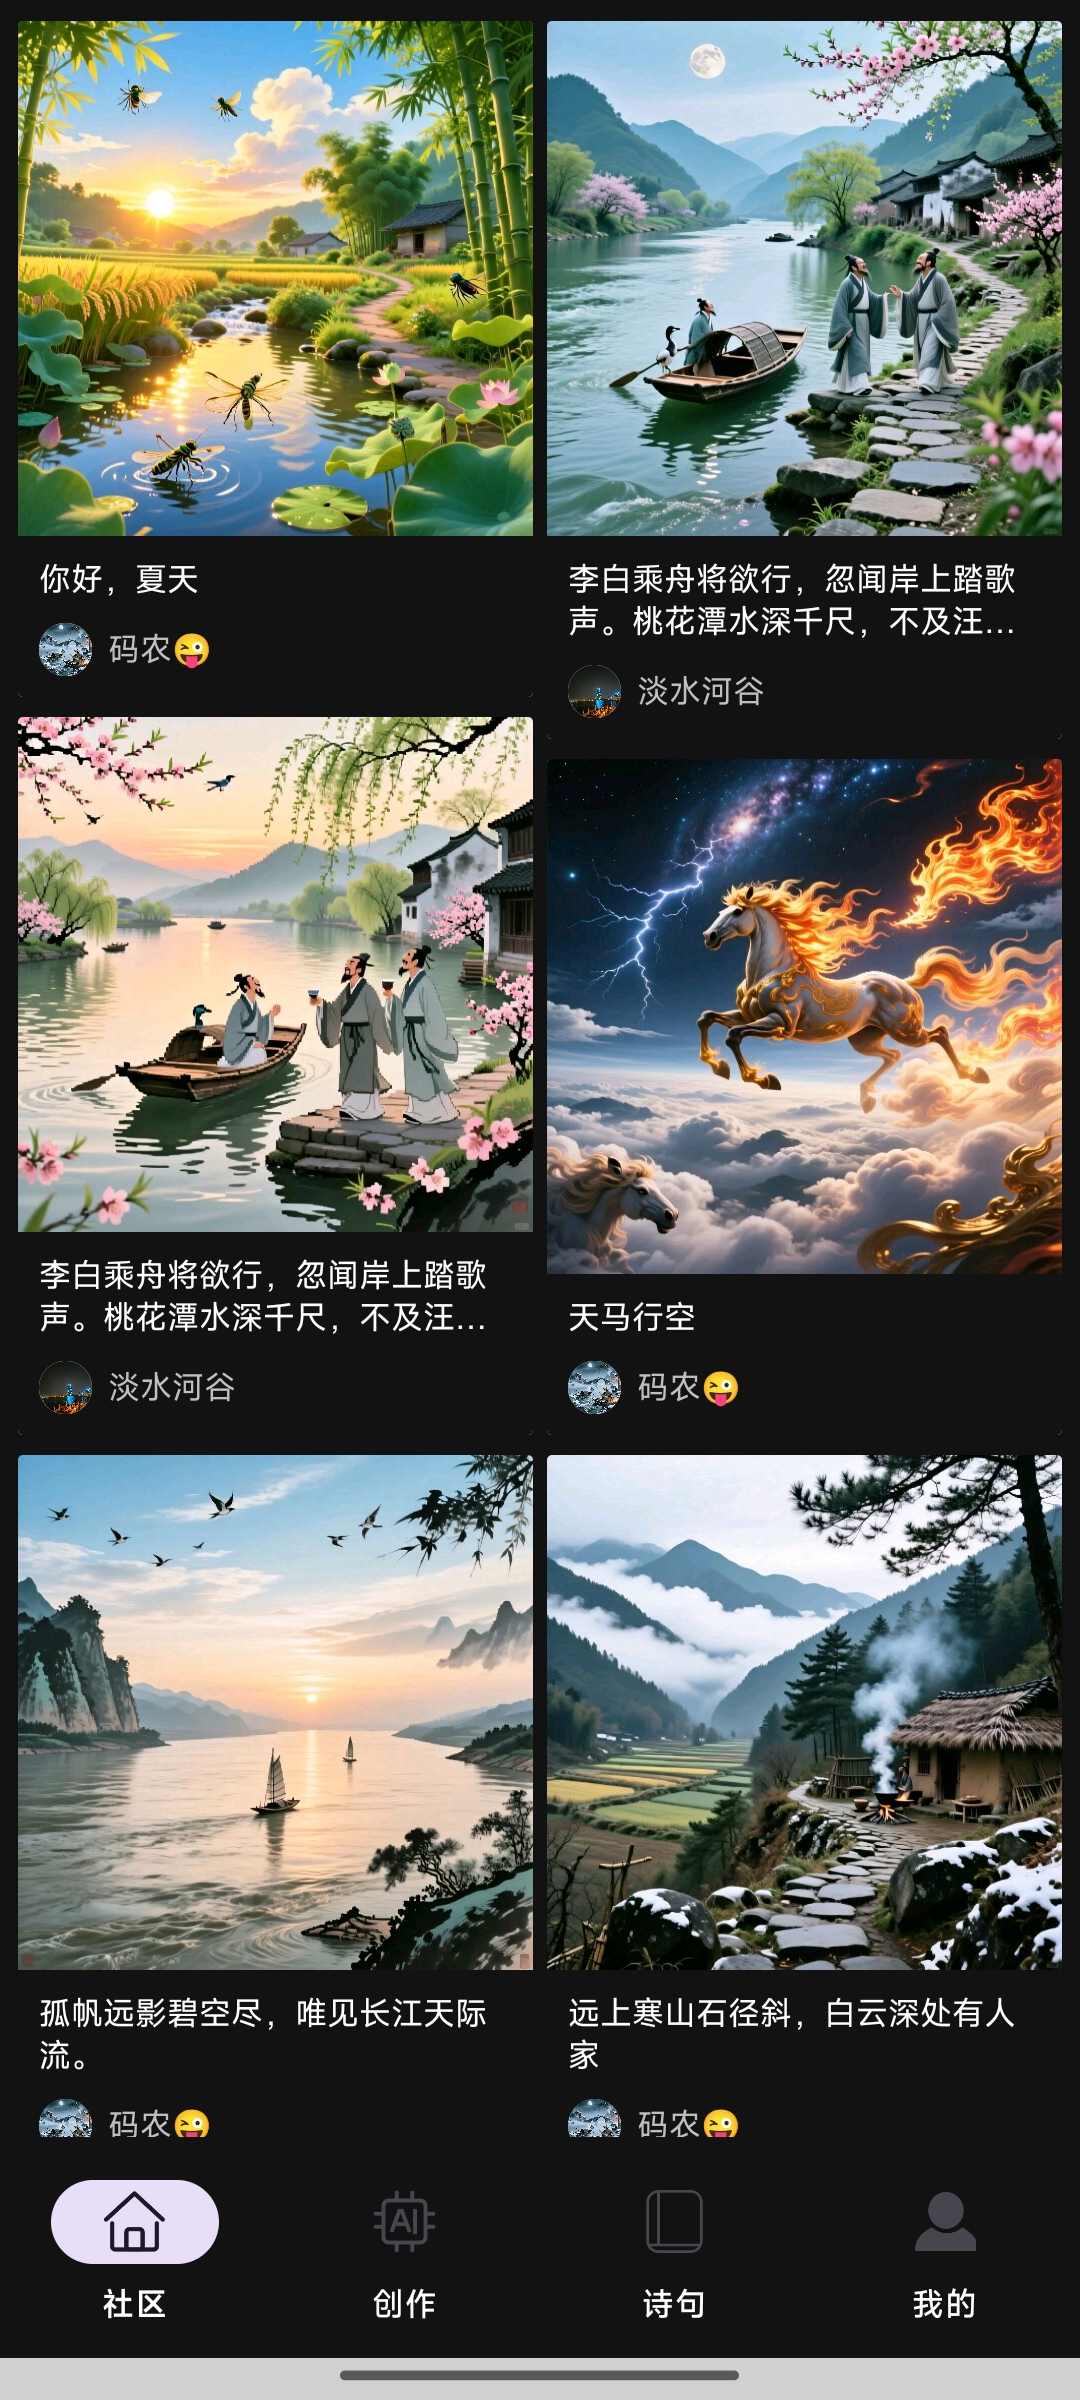
\includegraphics[height=3in]{figures/sec07_application/screenshots/20260416130204_722_194.jpg}
        % xiaojunhao
        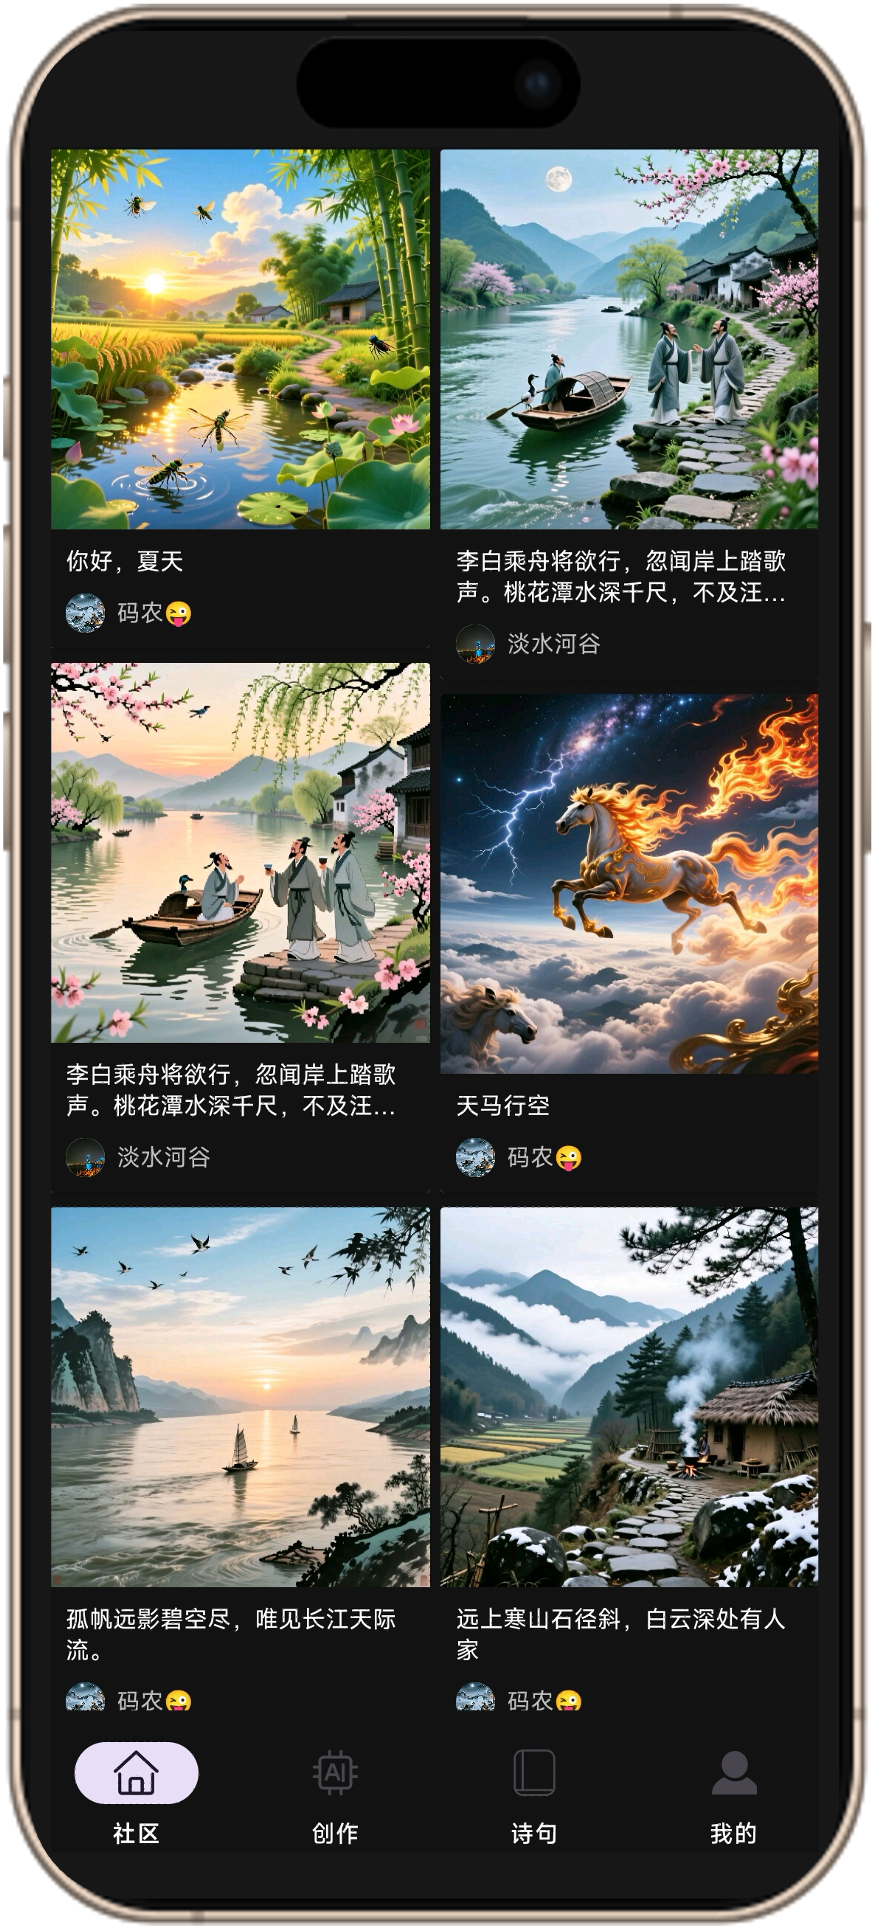
\includegraphics[height=3in]{figures/sec07_application/screenshots/a.png}
        \caption{Overview}
        \label{fig:mojie_overview}
    \end{subfigure}
    \hfill
    \begin{subfigure}[b]{0.23\linewidth}
        \centering
        % 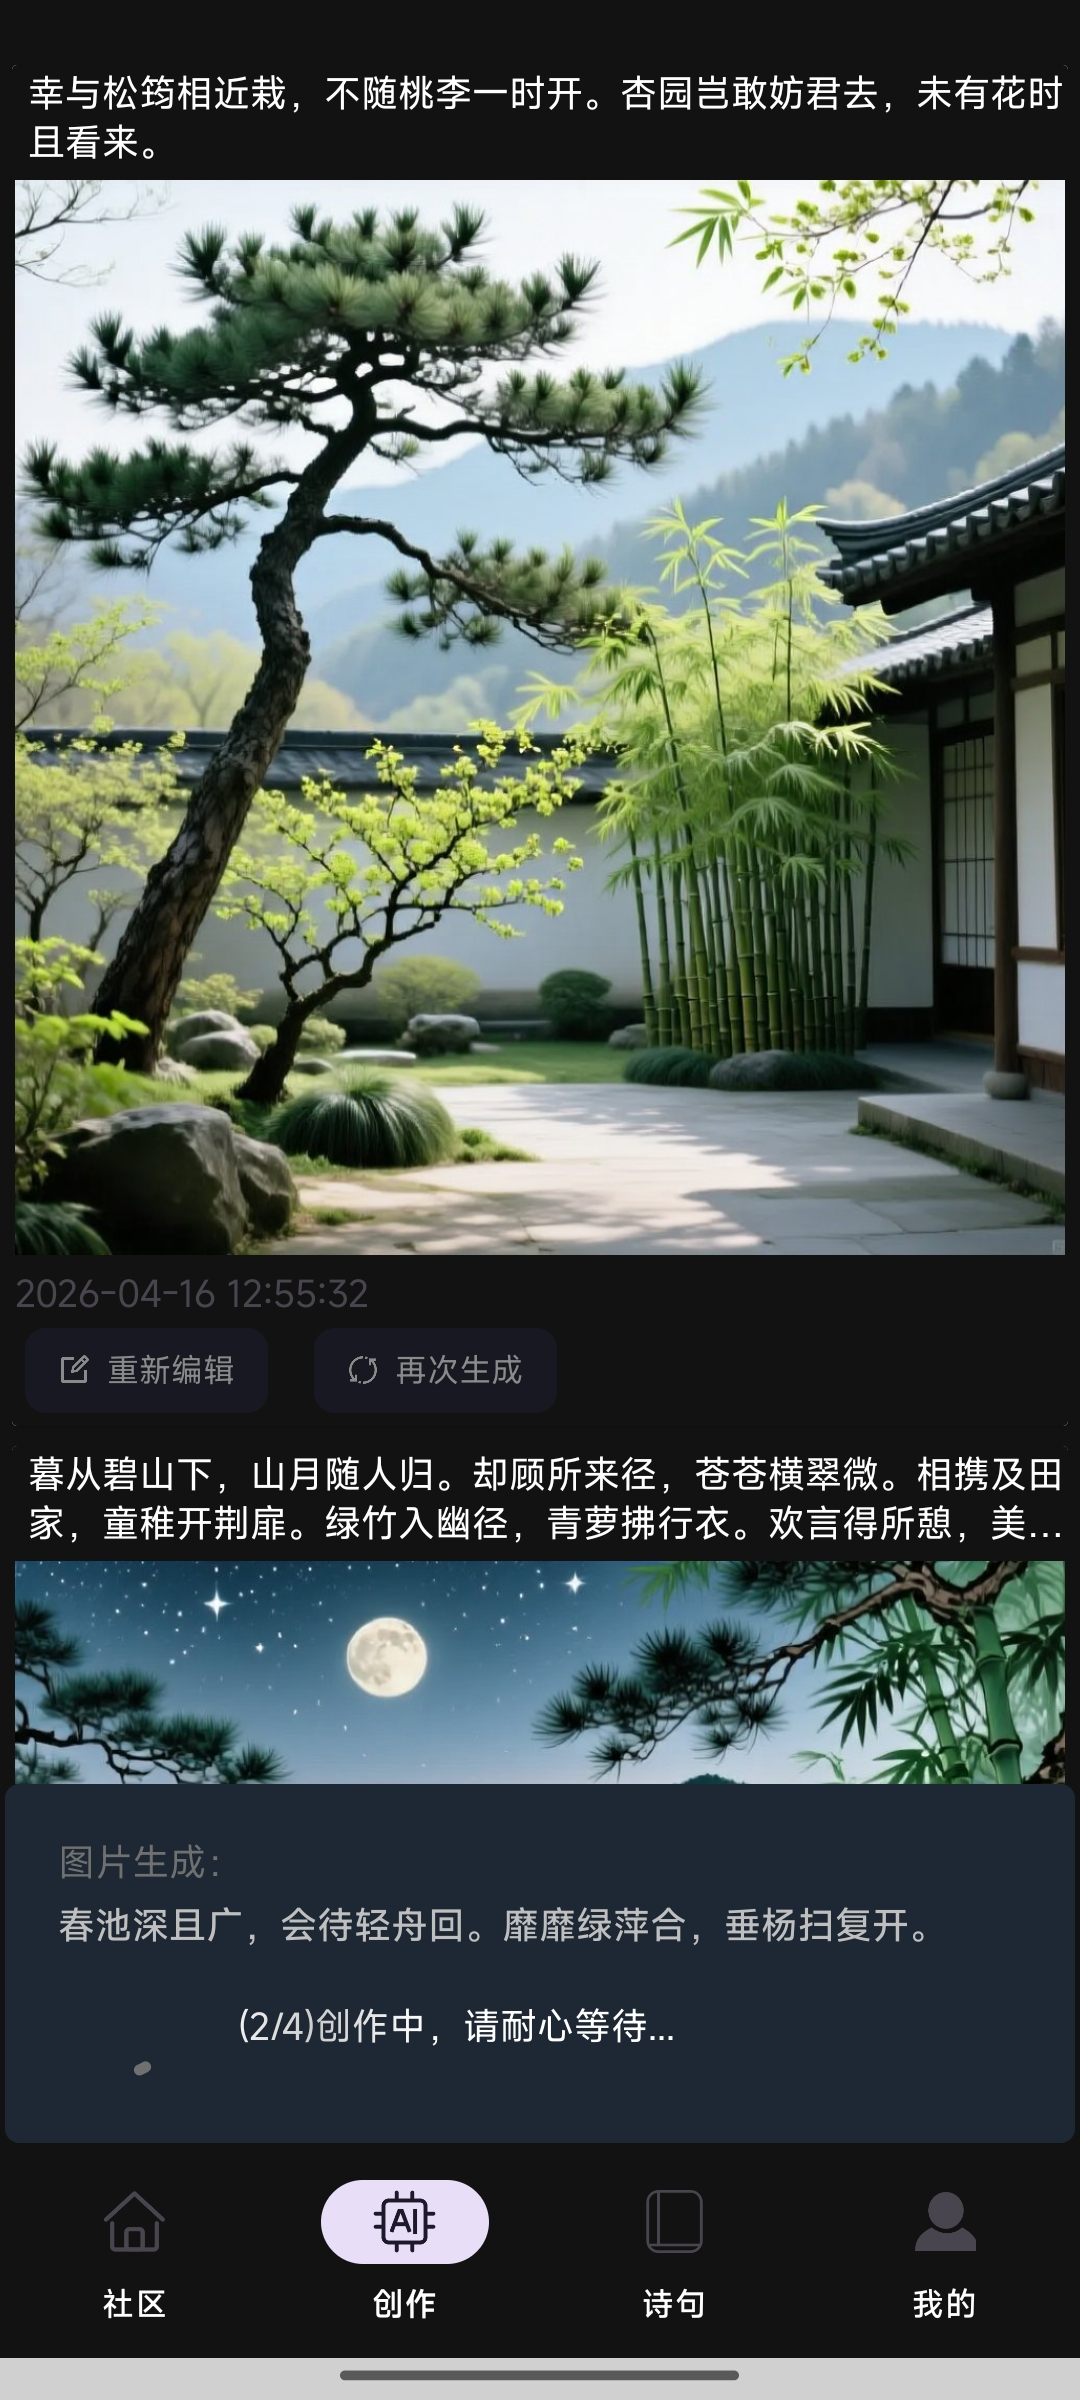
\includegraphics[height=3in]{figures/sec07_application/screenshots/20260416130210_728_194.jpg}
        % xiaojunhao
        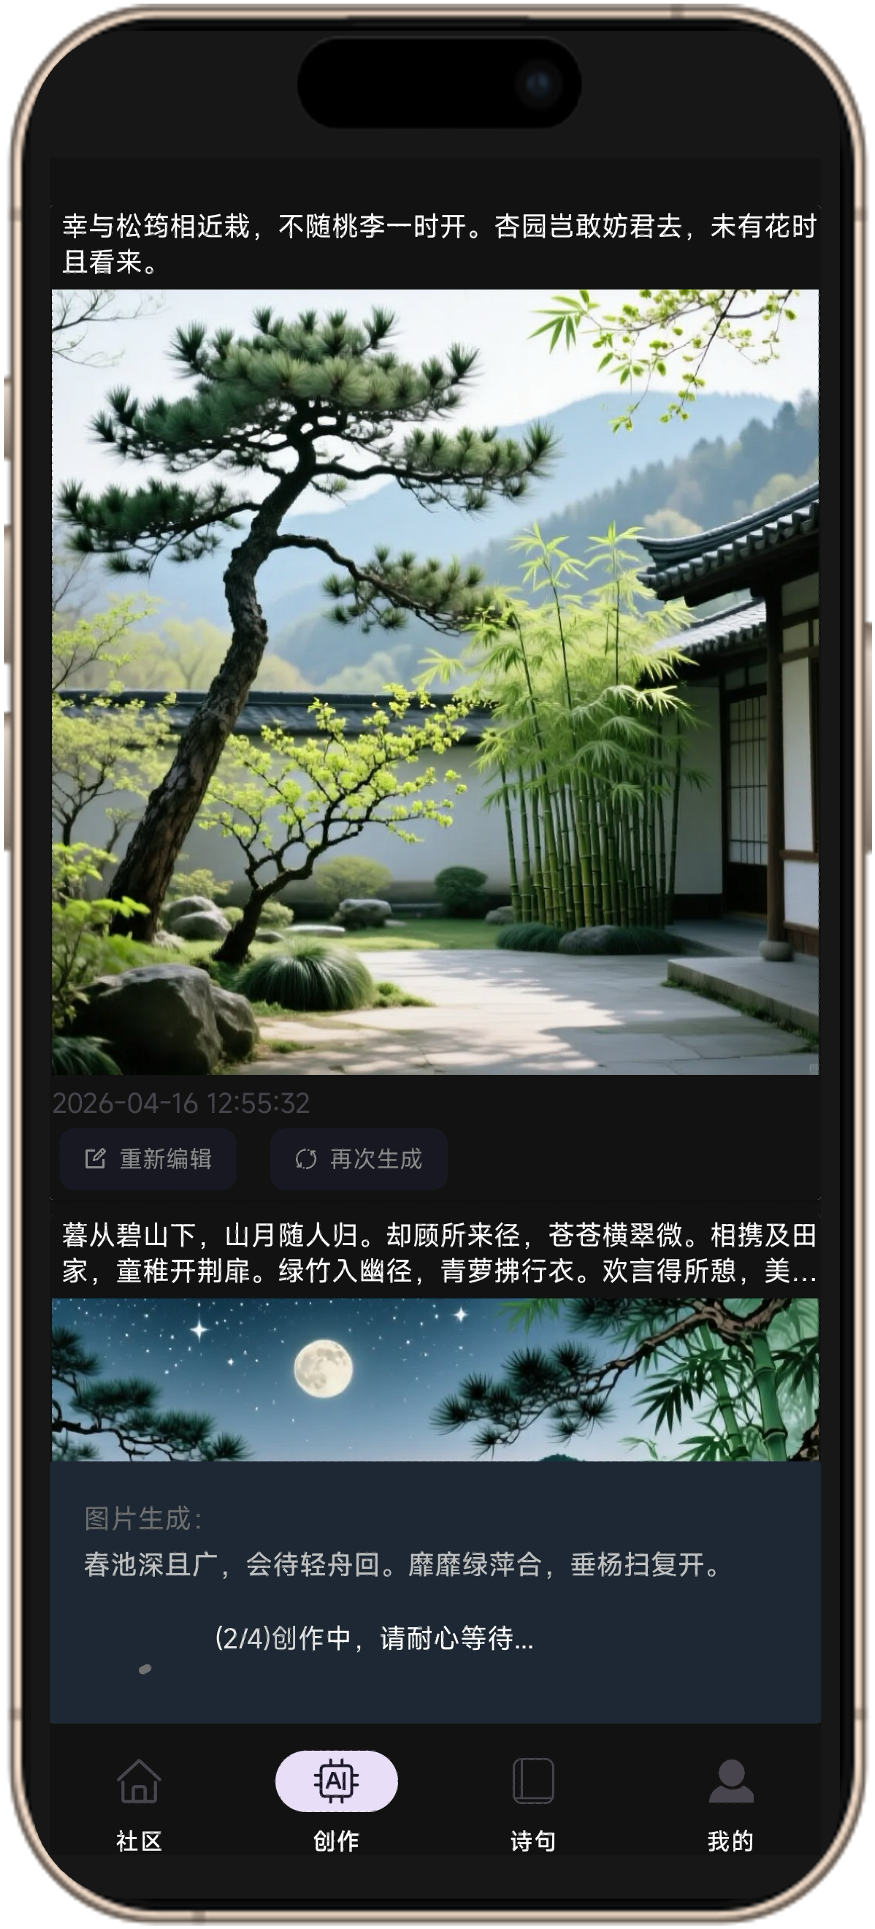
\includegraphics[height=3in]{figures/sec07_application/screenshots/b.png}
        \caption{Offline Generation}
        \label{fig:generation_in_mojie}
    \end{subfigure}
    \hfill
    \begin{subfigure}[b]{0.23\linewidth}
        \centering
        % 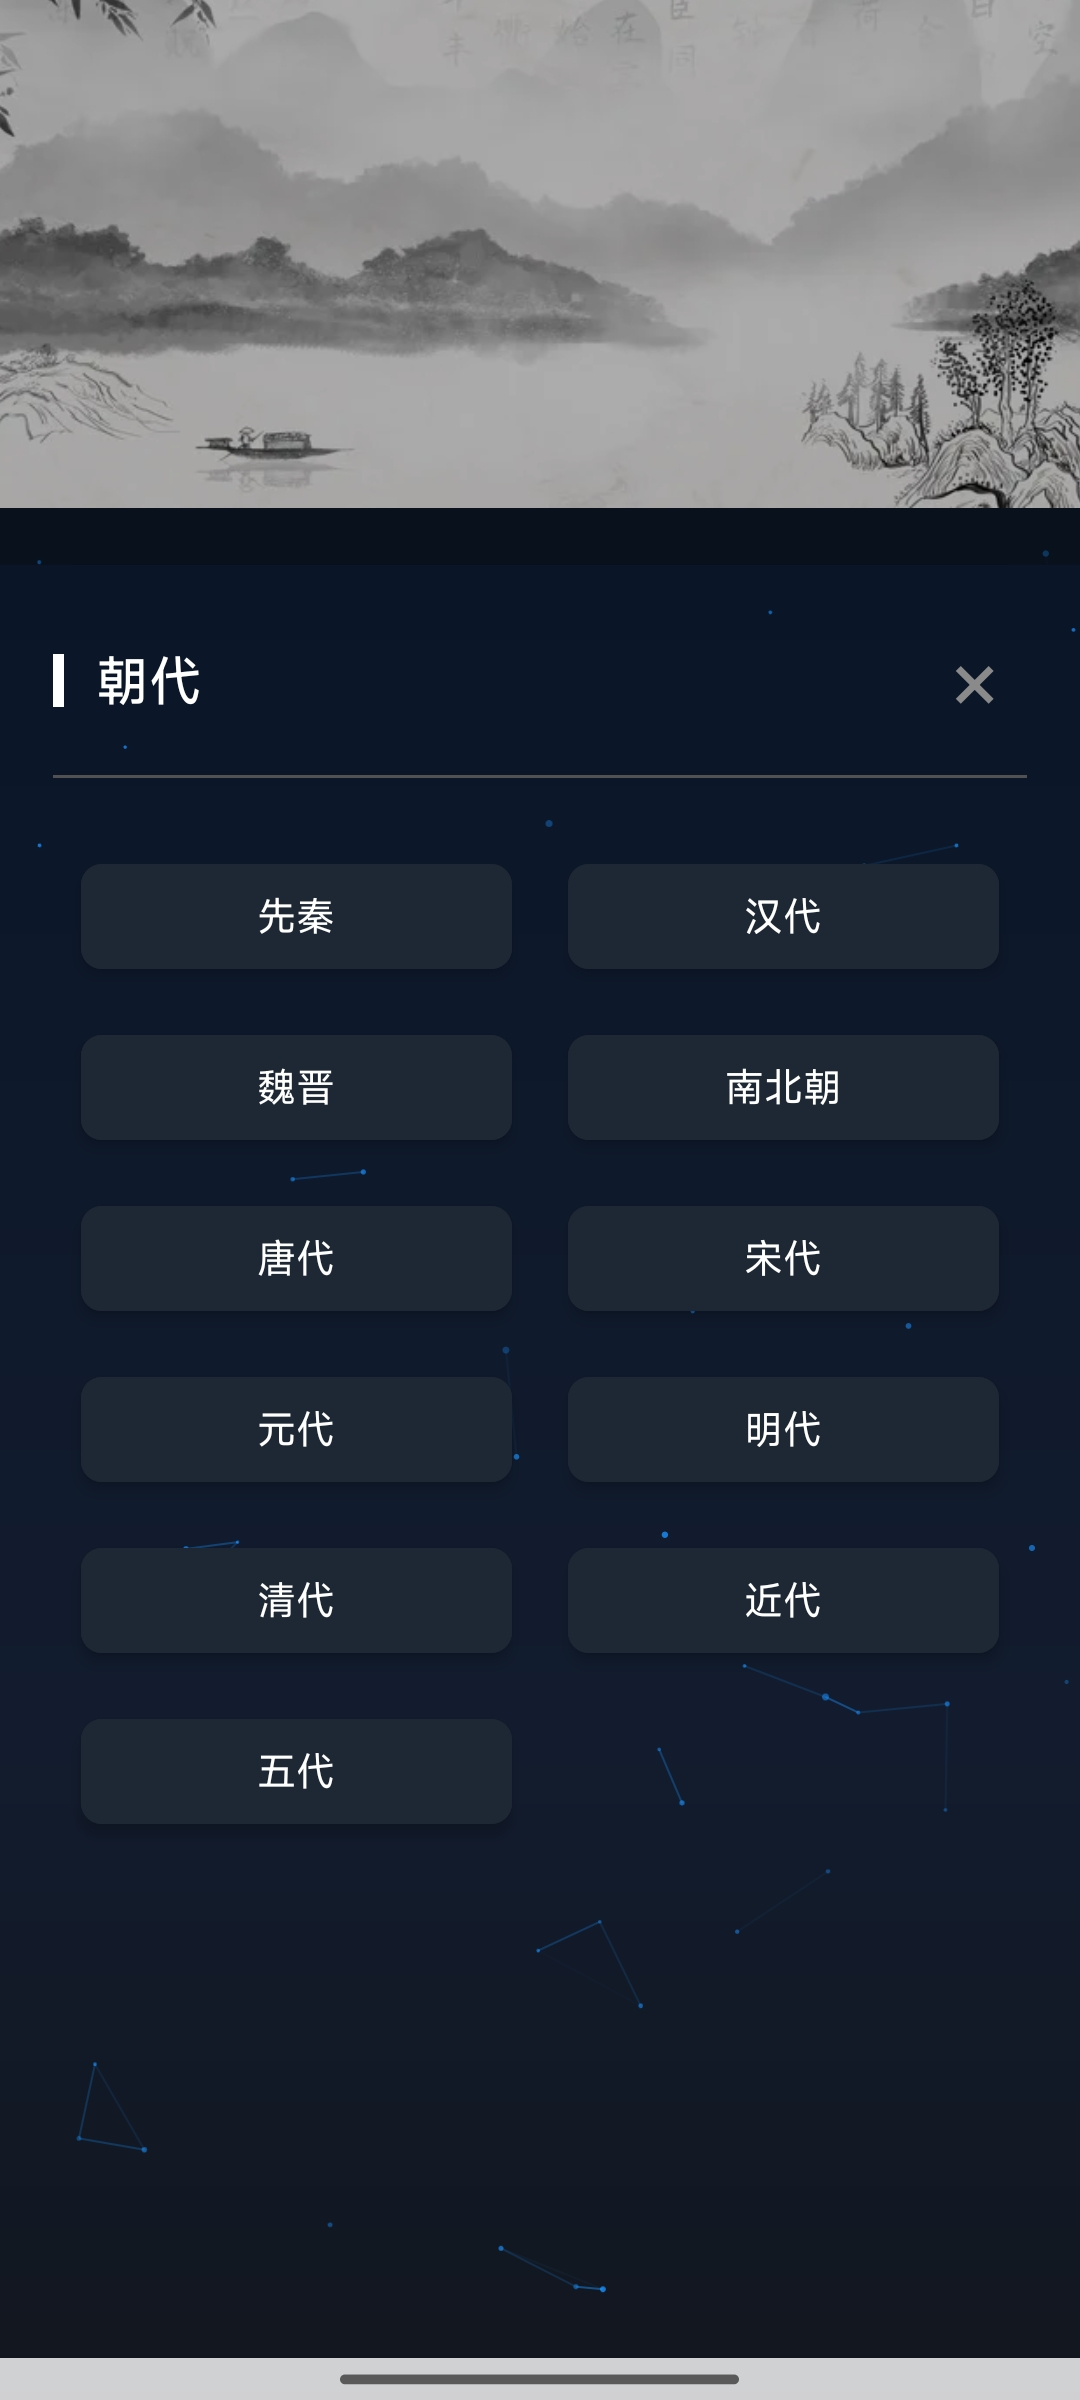
\includegraphics[height=3in]{figures/sec07_application/screenshots/20260416130212_730_194.jpg}
        % xiaojunhao
        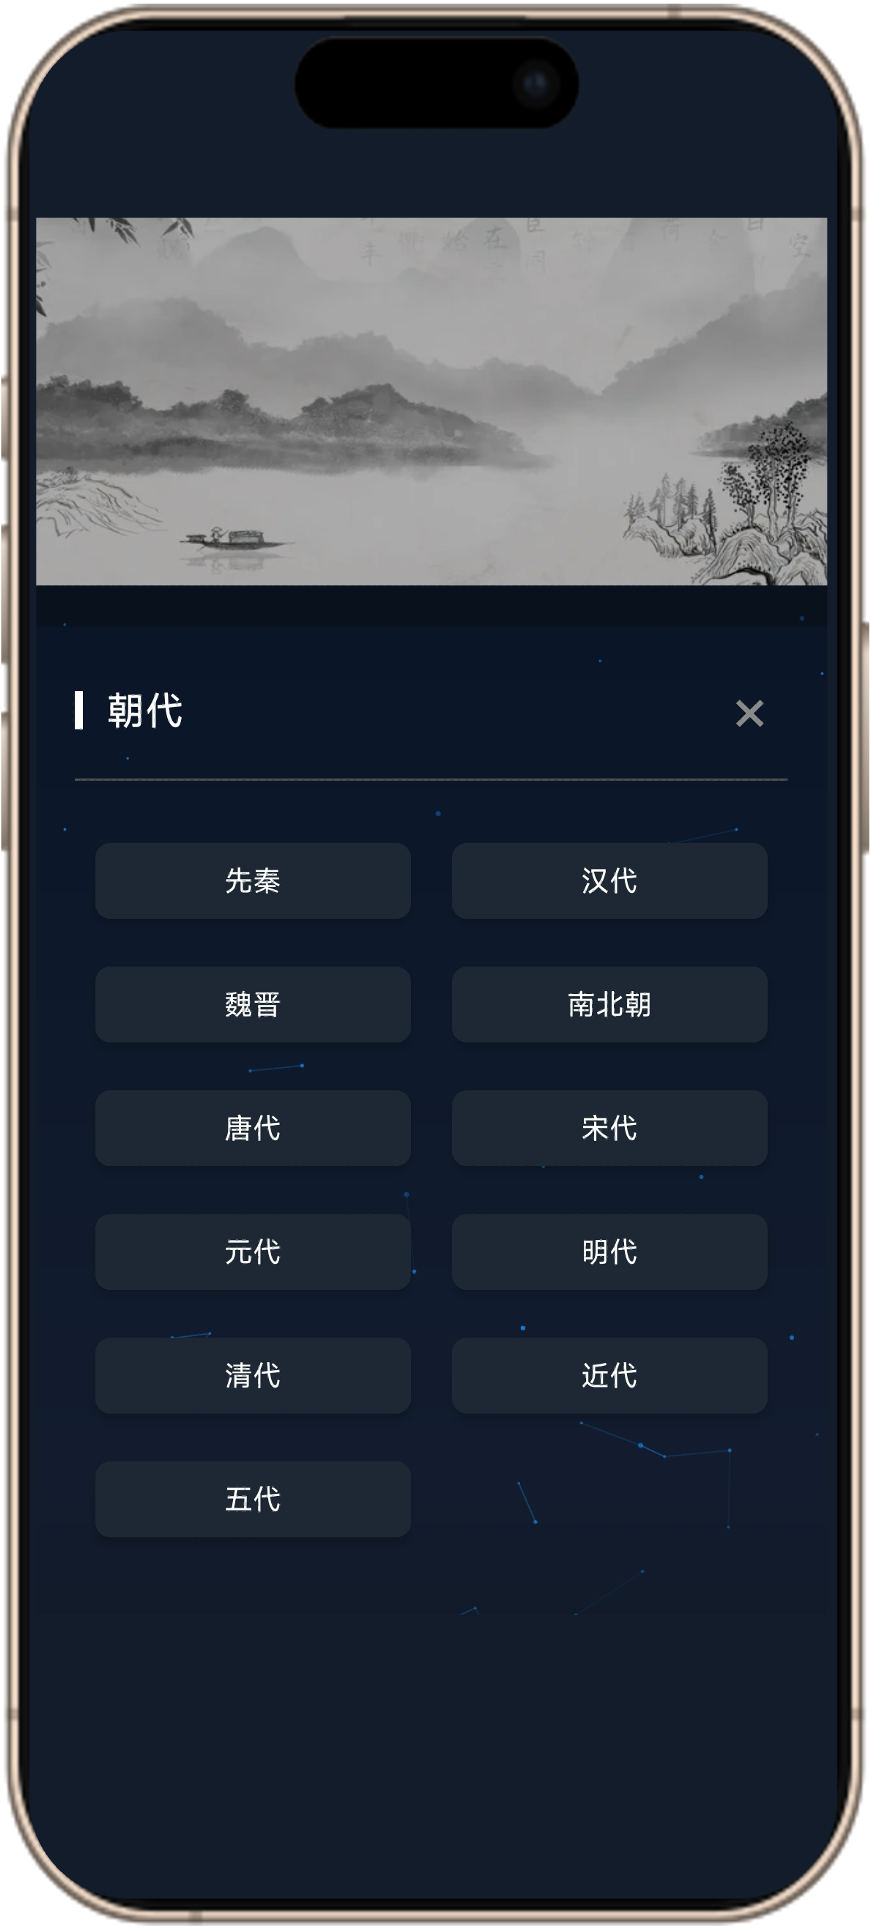
\includegraphics[height=3in]{figures/sec07_application/screenshots/c.png}
        \caption{Poetry Library}
        \label{fig:built_in_poetry_library}
    \end{subfigure}
    \hfill
    \begin{subfigure}[b]{0.23\linewidth}
        \centering
        % 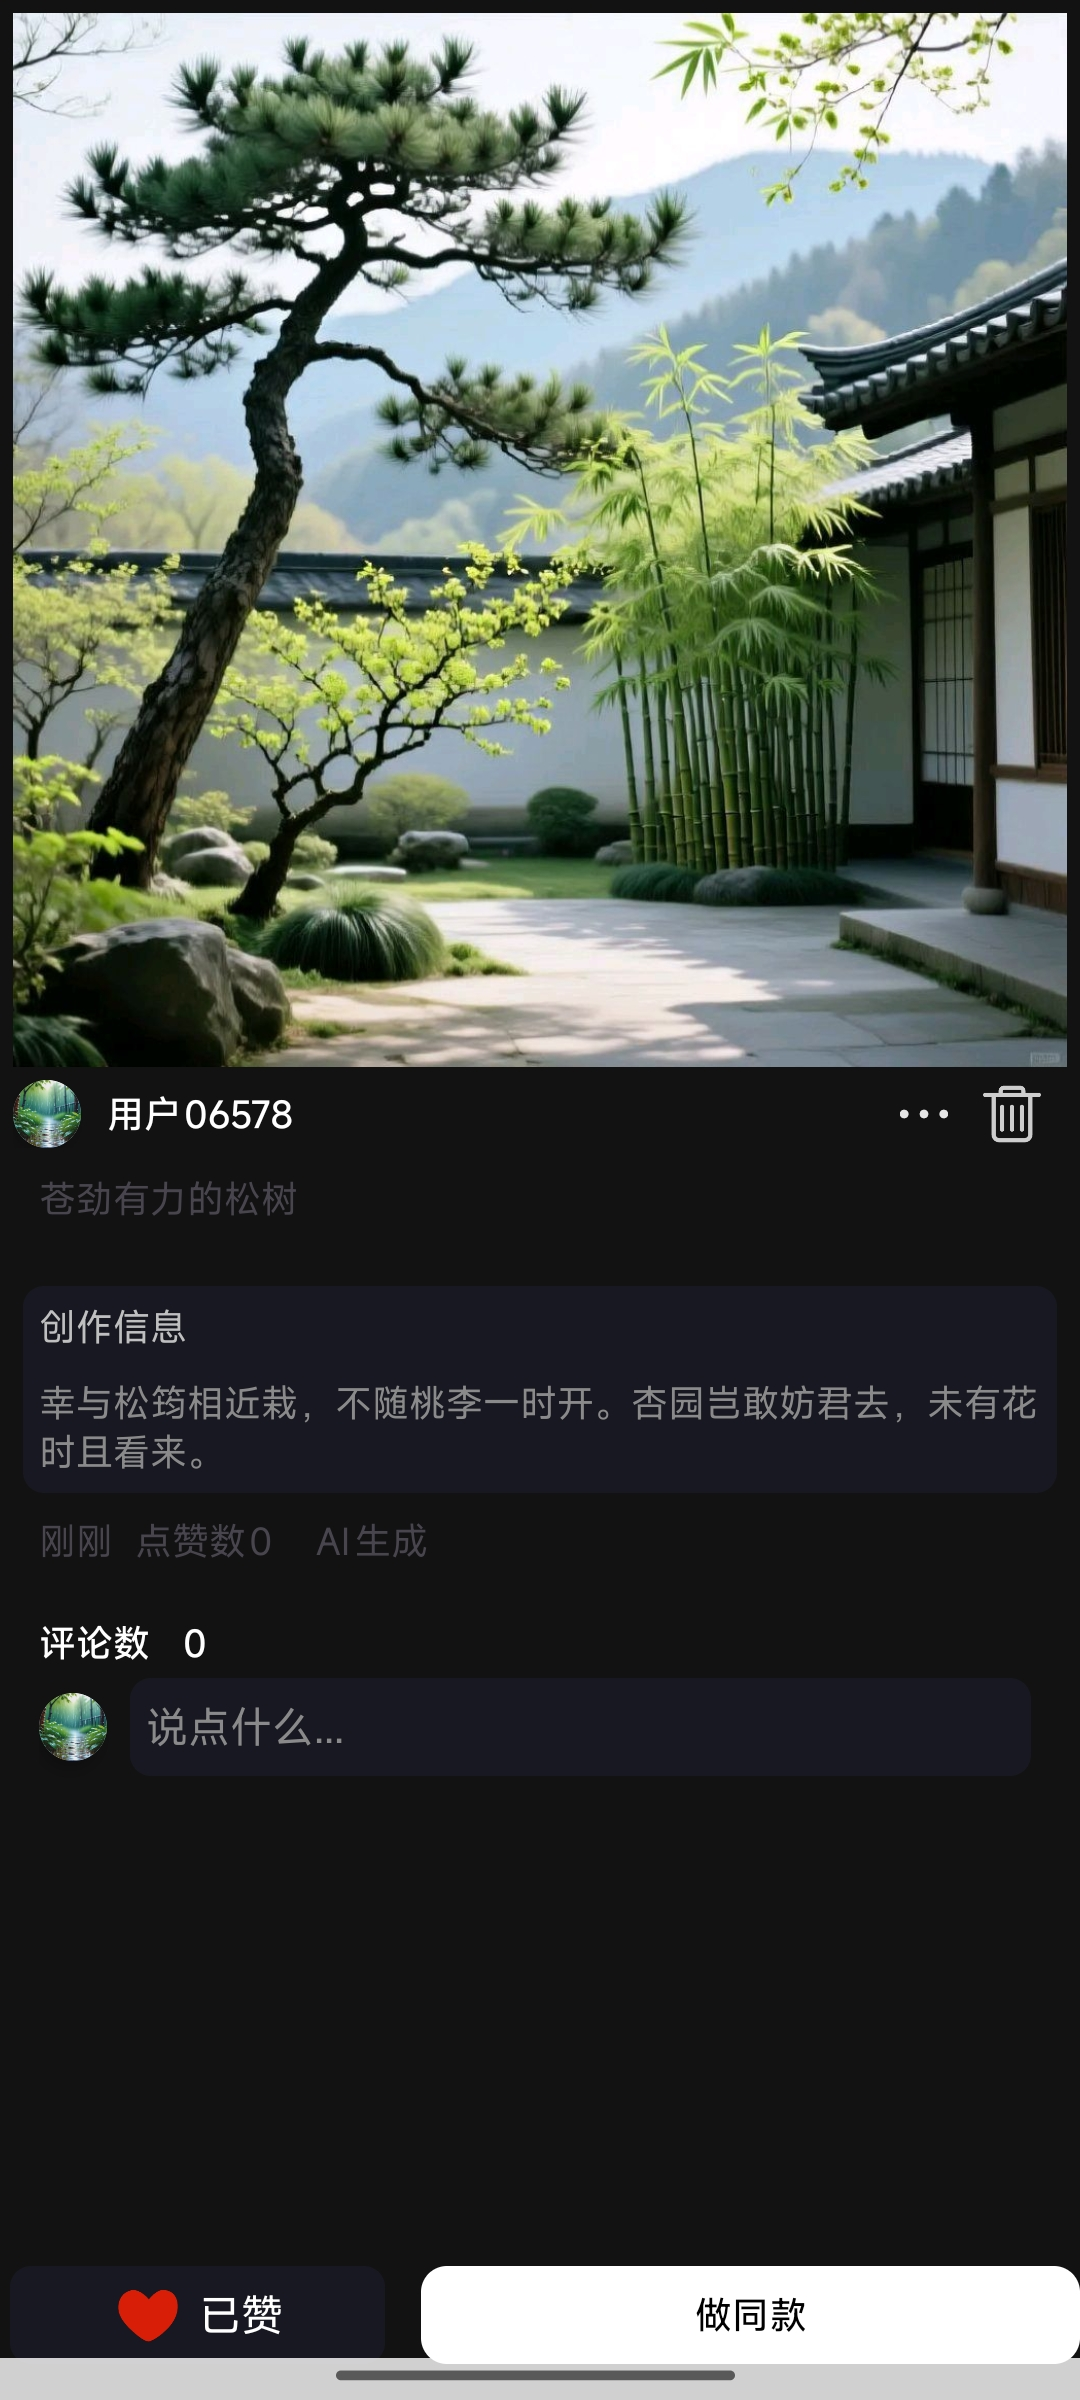
\includegraphics[height=3in]{figures/sec07_application/screenshots/20260416130216_734_194.jpg}
        % xiaojunhao
        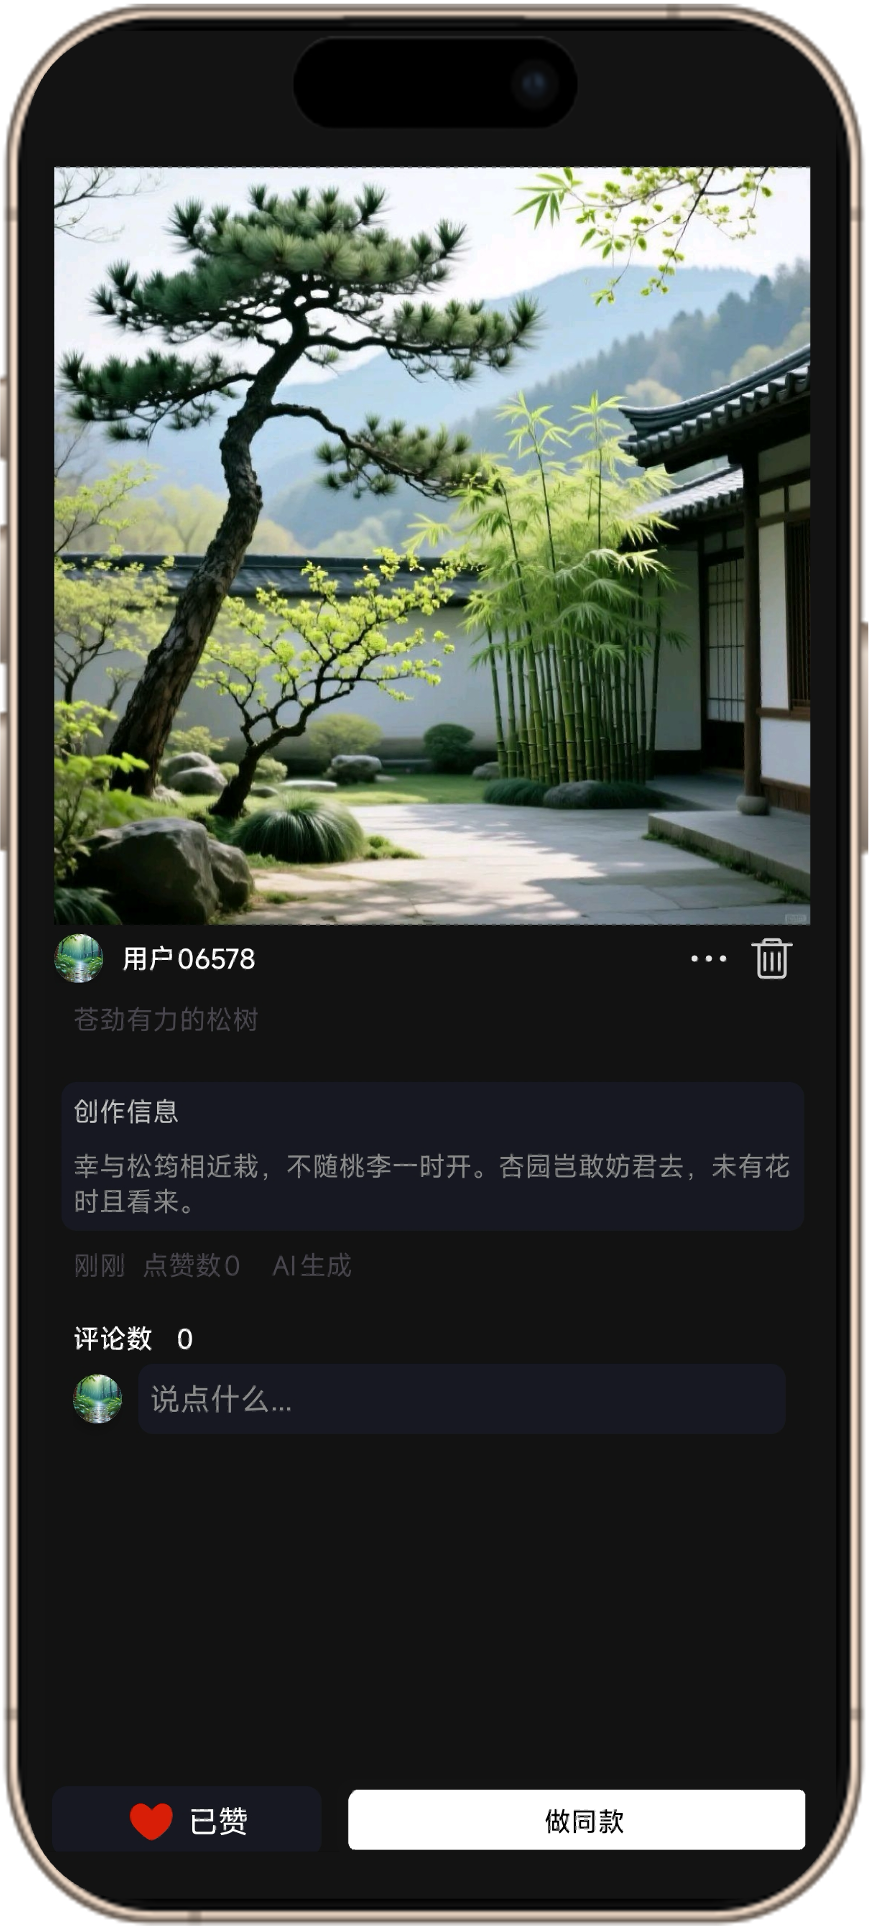
\includegraphics[height=3in]{figures/sec07_application/screenshots/d.png}
        \caption{Community}
        \label{fig:community_mojie}
    \end{subfigure}
    \caption{Screenshots of the Mojie application on Android devices, illustrating (a)~the main interface, (b)~offline poetry-to-image generation, (c)~the built-in classical poetry library, and (d)~community sharing and social interaction.}
    \label{fig:mojie_screenshots}
\end{figure}

\subsubsection{iOS application integration and runtime execution}

On the application side, we implement an iOS app in Swift that uses the Core ML framework to load and invoke the converted models. During inference, the input text is first encoded by CLIP, the latent representation is iteratively denoised by U-Net, and the final image is reconstructed by the VAE decoder. This execution order preserves the original structure of the diffusion pipeline while enabling the full three-model generation branch to run natively on iPhone.

Compared with the Android deployment, which partitions execution across MNN and QNN, the iOS implementation uses a unified Core ML runtime for both model invocation and inference. This unified deployment path simplifies software integration and demonstrates that the JuZhou 1.0 diffusion backbone can be migrated to the Apple mobile ecosystem without modifying its core model architecture.

\subsubsection{Experimental results on iPhone}

We evaluate the Apple-side deployment on an iPhone 15 Pro equipped with the A17 Pro chip. Tab.~\ref{tab:hardware_profiling} further profiles the denoising network at 1024 $\times$ 1024 resolution on flagship mobile platforms, showing that JuZhou 1.0 remains executable under practical mobile memory and latency constraints, whereas mainstream SD 1.5 and SDv2.1 baselines fail under the same on-device setting. 
In this implementation, CLIP, U-Net, and VAE all run in FP16 without additional quantization. The total runtime memory footprint is 373\,MB, and the latency of a 4-step diffusion run is 4.25\,s.
These results confirm that the three-model diffusion stack can be executed natively on current iPhone hardware without post-training quantization. Although the present Apple-side validation does not yet include the auxiliary prompt-refinement language model, it demonstrates that the core image-generation path of JuZhou 1.0 is already deployable and operational on iOS devices.

\subsection{Cross-platform implications}
Taken together, the Android and iOS results demonstrate that JuZhou 1.0 can be deployed across heterogeneous mobile ecosystems through platform-specific toolchains while preserving the same high-level model decomposition. Android emphasizes engine-level partitioning between MNN and QNN, whereas iOS relies on a unified Core ML stack.
This cross-platform evidence shown in Fig.~\ref{fig:latency_comparison} is significant for edge-AI deployment because it indicates that the same poetry-to-image architecture can adapt to different mobile hardware and software environments without redesigning the model itself. The Apple-side result further shows that an unquantized FP16 diffusion branch can still achieve practical latency on flagship phones.
\footnotetext{``--'' denotes model failure due to excessive VRAM requirements or extreme latency exceeding practical utility. JuZhou 1.0 metrics cover the denoising network only: MACs 579.65\,G and FLOPs 1161.82\,G. CLIP and VAE overheads are excluded.}



